\documentclass[11pt,a4paper,twoside]{article}
\usepackage[dutch]{babel}
%laad de pakketten nodig om wiskunde weer te geven :
\usepackage{amsmath,amssymb,amsfonts,textcomp}
%laad de pakketten voor figuren :
\usepackage{graphicx}
\usepackage{float,flafter}
\usepackage{hyperref}
\usepackage{inputenc}
\usepackage{listings}
%zet de bladspiegel :
\setlength\paperwidth{20.999cm}\setlength\paperheight{29.699cm}\setlength\voffset{-1in}\setlength\hoffset{-1in}\setlength\topmargin{1.499cm}\setlength\headheight{12pt}\setlength\headsep{0cm}\setlength\footskip{1.131cm}\setlength\textheight{25cm}\setlength\oddsidemargin{2.499cm}\setlength\textwidth{16.5cm}

\begin{document}
\begin{center}
{\bf {\Huge UNIVERSITY OF VICTORIA} ~\\
	~\\
	{\huge Department of Electrical and Computer Engineering} ~\\
	~\\
	~\\
	{\huge ECE 403/503 Optimization for Machine Learning} ~\\
	~\\
	~\\
	~\\
	{\huge LABORATORY REPORT}
	~\\
	~\\
	~\\
}
\end{center}
{\bf
{\LARGE Experiment No: 04}
~\\
~\\
~\\
{\LARGE Title: Breast Cancer Diagnosis via Logistic Regression}
~\\
~\\
~\\
{\LARGE Date of Experiment: 16 July, 2019}
~\\
~\\
~\\
{\LARGE Report Submitted on: 23 July, 2019}
~\\
~\\
~\\
{\LARGE To: Mr. J. Zhan}
~\\
~\\
~\\
{\LARGE Laboratory Group No.: B01 T 12}
~\\
~\\
~\\
{\LARGE Name(s): Alvi Mahadi (V00912845)}
~\\
~\\
~\\
}

\newpage
% !TEX root = main.tex
\section{Introduction and Objectives}
\label{sect:introduction}
In this experiment, we investigate a technique for multi-category classification based on binary
classifications. The technique is then applied to Fisher`s 3-class datasets of Iris plants to
demonstrate its effectiveness. The dataset of Iris plants to be used in this experiment was created
and published in 1936 by R. A. Fisher [1]. Fisher's paper is a classic in the field and is referenced
frequently to this day, as a matter of fact the dataset is arguably the best-known in the pattern
recognition literature [2]. The dataset includes features of 150 Iris plants of 3 species known as
Setosa, Versicolor, and Virginica, where each sample Iris is represented by a 4-dimensional vector
in terms of lengths and widths of the sepal and petal of the flower.
% !TEX root = main.tex
\section{Implementation Steps and Results}
\label{sect:implementation-result}

\subsection{Implementation Steps}
\label{subsect:implementation_steps}
We strictly followed the implementation steps stated in the laboratory manual [3].

\subsection{Code}
\label{subsect:code}

\begin{lstlisting}[language=Matlab]
clc;
clear all;
close all;
D_tr = load('/home/alvi/Documents/courses/ece503/labs/3/data/D_build_tr.mat');
Xtr = D_tr.D_build_tr(1:8,:);
Ytr = D_tr.D_build_tr(9:10, :);
D_te = load('/home/alvi/Documents/courses/ece503/labs/3/data/D_build_te.mat');
Xte = D_te.D_build_te(1:8,:);
Yte = D_te.D_build_te(9:10, :);
Xtr = [Xtr' ones(640, 1)];
I = eye(9);
W_B = pinv(Xtr' * Xtr + 0.01 * I) * Xtr' * Ytr';
W = [W_B(1:8, 1) W_B(1:8, 2)];
b = W_B(9, :)';
e_p = double.empty();
Y = double.empty();
for i=1:128
y = W' * Xte(:, i) + b;
Y = [Y, y];
end
e_p = norm(Yte - Y, 'fro') / norm(Yte, 'fro');
disp(e_p);
I = 1:128;
plot(I, Yte(1, I), 'r', I, Y(1, I), 'g');
plot(I, Yte(2, I), 'r', I, Y(2, I), 'g');
\end{lstlisting}

\subsection{Result}
\label{subsect:result}
\begin{figure}[h]
	\centering
	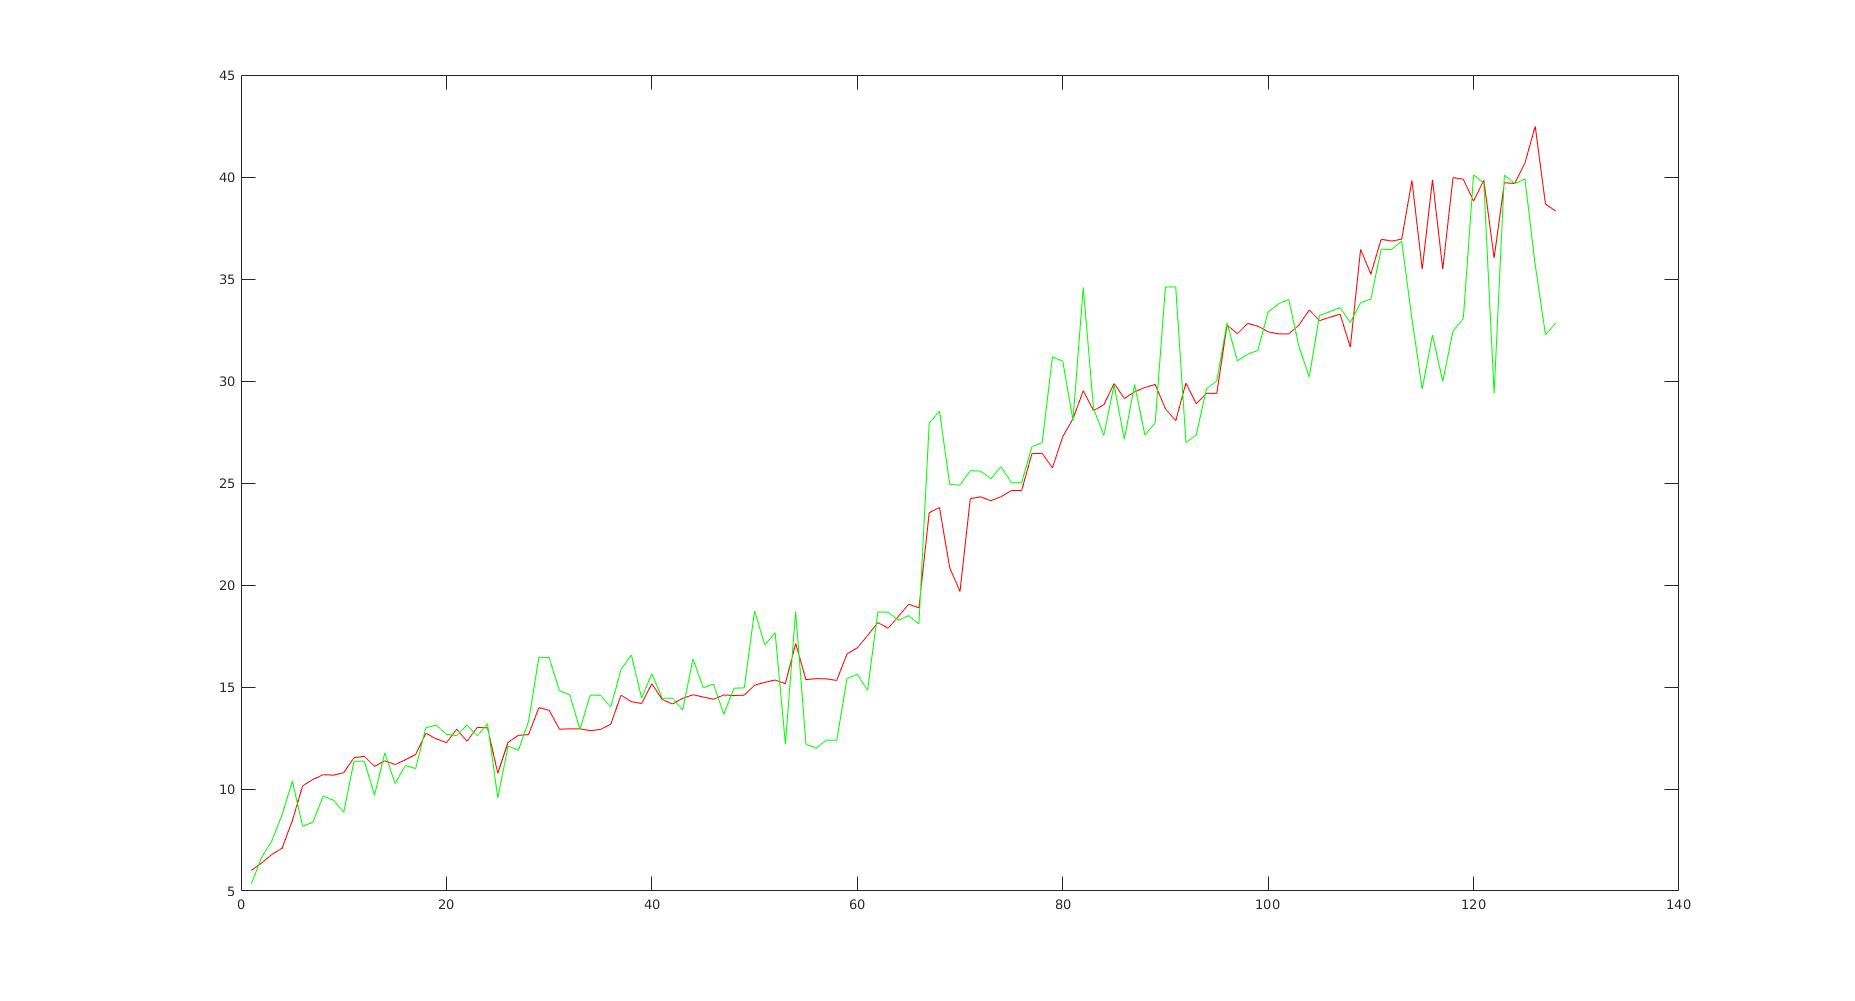
\includegraphics[width=\textwidth]{/home/alvi/Documents/courses/ece503/labs/3/result/1.jpg}
	\caption{First row of $Yte$ and first row of $Y^{(p)}$}
	\label{fig:1}
\end{figure}

\begin{figure}[h]
	\centering
	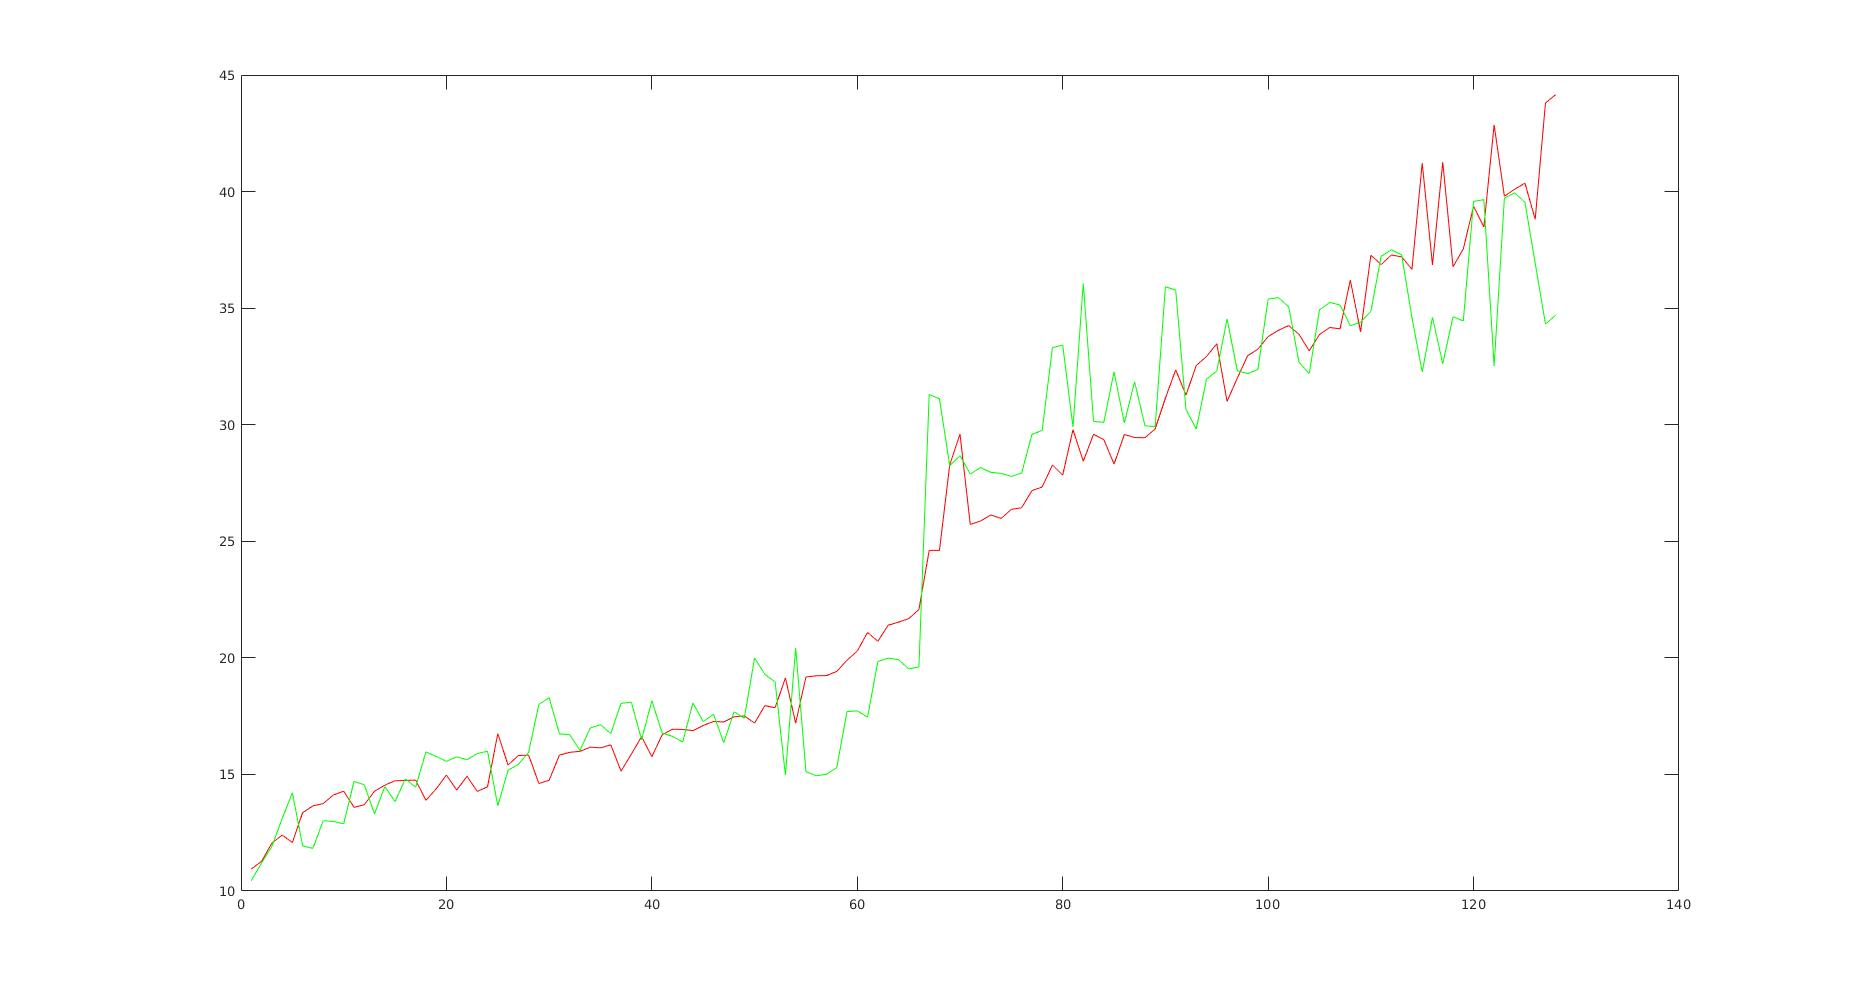
\includegraphics[width=\textwidth]{/home/alvi/Documents/courses/ece503/labs/3/result/2.jpg}
	\caption{Second row of $Yte$ and second row of $Y^{(p)}$}
	\label{fig:1}
\end{figure}
\end{document}